\documentclass{iSWAGArticle}

%\usepackage{lipsum}
\usepackage{amssymb}
\usepackage[dvips]{epsfig,psfrag}
\usepackage[utf8]{inputenc}

\title{In-Rank mesh optimization for URL customized promotion in SEO}
\author{\iSWAGAuthor{Stefan Duprey\\
Cdiscount\\
stefan.duprey@cdiscount.com} \and \iSWAGAuthor{Second Author\\
Second University\\
second.author@university2.com}}

\begin{document}

\maketitle

\begin{abstract}
 Web site internal mesh optimization is at the very heart of search engine optimization. 
 One prominent way to get the best web search engine visibility for our site 
 is to build the adequate internal linking to promote our naturally popular pages. 
 The definition of popular might be the transformation rate for e-commerce, 
 the traffic from logs for a common site or even a semantic quality rate for our page. 
 We here propose an algorithm to automatically compute the optimal internal mesh for our web site.
 We tackle the challenges met both at a theory and software implementation level. 
 We'll more specifically deal with big data issues for an e-commerce web site.
 \\\newline
 \indent \textbf{Keywords: }
 \\\newline
search engine, e-commerce, page rank, in rank, mesh optimization, global optimization
\end{abstract}

\section{Introduction}
We here propose an original methodology to optimize the internal mesh of Cdiscount e-commerce site.
The idea behind is to promote the most successful URLs (the most frequently viewed by users) by increasing their in-rank.  
The frequency data is obtained from logs parsing tracking software and the in rank is computed using the famous page rank iterative algorithm.  
We want to find the optimal mesh, which maximizes for all URLs the matching between their traffic and their in-rank. 
The more successful a URL is, the more in-rank we want to give him through our optimal mesh.
 \\\newline
We here detail the technical implementation of such an algorithm.
The difficulty here is three-fold:
\\
\indent
First the structure of an e-commerce is already well-defined and it is out of question to drastically change the already existing mesh.
Links are categorized regarding their incoming page type and position within that page and links can only be created within certain categories. 
So we'll have strong constraints for our mesh to comply with.
\\
\indent
Second the universe we deal with is discrete and gigantic. 
For a mesh with $N$ nodes, the number of possible meshes is $2^{N^{2}}$. 
Our objective function is non-linear and non-convex. Exhaustive optimization would be far too computationally intensive. 
We have to find a proper heuristic based global optimization algorithm to cleverly tweak through our universe.
\\
\indent
Third the actual size of our data makes the implementation of a real-world industrial use case a technologically difficult problem.
Either we implement from scratch over a cluster our algorithm dealing ourselves with concurrency and inter-processor communications,
or we try not to reinvent the wheel and plug ourselves to existing big data platform.
The double iterative nature of our algorithm (page rank computations and optimization are both naturally iterative)
makes Hadoop Map/Reduce paradigm too slow for our purpose. 
In contrast to Hadoop's two-stage disk based Map/Reduce paradigm, Spark's in-memory primitives provide the needed performance.
By allowing user programs to load data into a cluster's memory and query it repeatedly, Spark is well suited for our purpose.
We'll detail the technological implementation of a real-world use case.

\section{Algorithm}
Let $N \in \mathbb{N}$ be the number of nodes of our graph or rather the number of URLs of our site.
 \\\newline
Let's $$\left(X_i\right)_{i \in \left\{1,...,N\right\}}$$ denote the nodes of our directed graph.
 \\\newline
Let's $$\left(G_{ij}\right)  \in \left\{0,1\right\}^{N\times N}$$ denote the adjacency matrix of our directed graph.



Genetic algorithm is a search heuristic that mimics the process of natural selection 
A population of individuals to an optimization problem is evolved toward better solutions. 

In our case, each individual or chromosome $\left(C_{ij}\right)  \in \left\{0,1\right\}^{N\times N}$ here represented as a bits array, which results from the vectorization of
the adjacency matrix $\left(G_{ij}\right)$


A candidate can either result from a crossover between two parents or from a self mutation;
The crossover function which breeds a child from two parents is defined as follows :
The child will keep the matching bits of the two parents and inherit randomly every other non-matching bits.
For every two parents, we spawn two children :
\\\newline
\textbf{\large Child spawn from 2 parents crossover}
\begin{center}
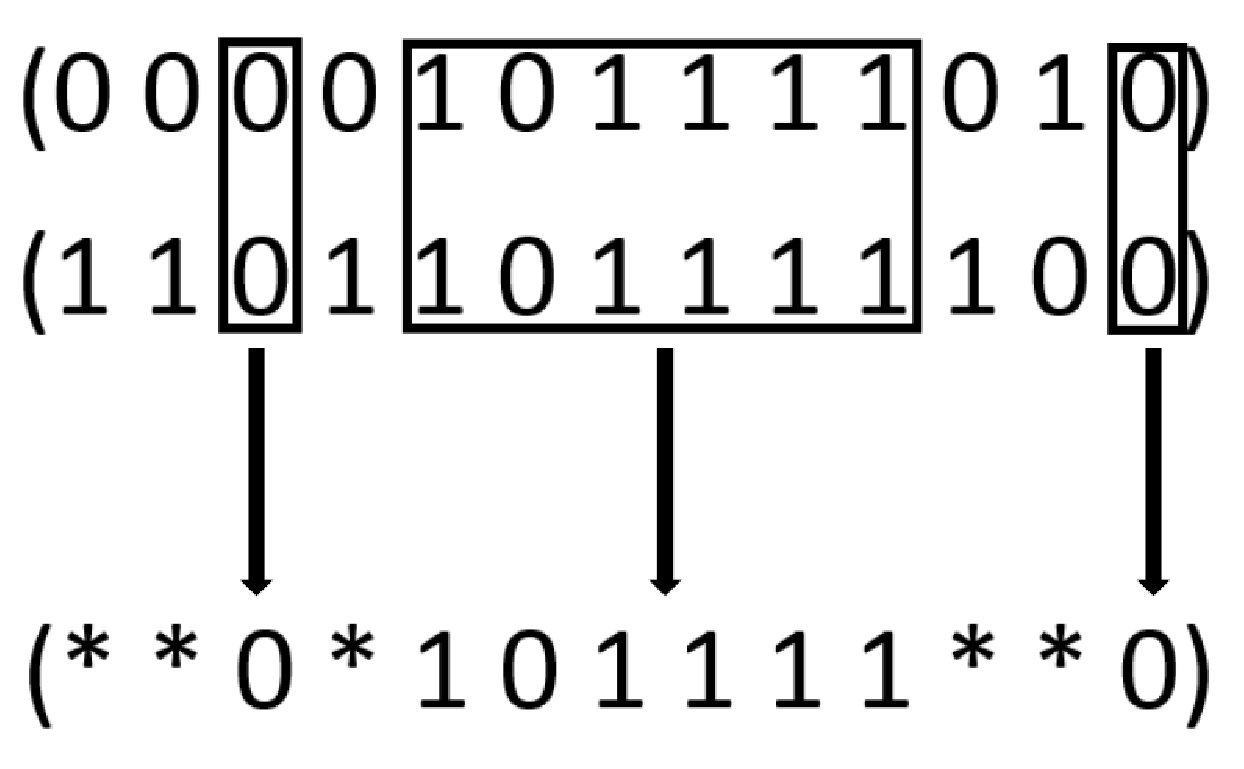
\epsfig{file=crossover.eps,height=2cm,width=4cm}
\end{center}
The mutation function is even simpler : we just switch bits whose locations are randomly chosen
and proportions equal a fixed mutation rate : 
\\\newline
\textbf{\large Mutation of an individual}
\begin{center}
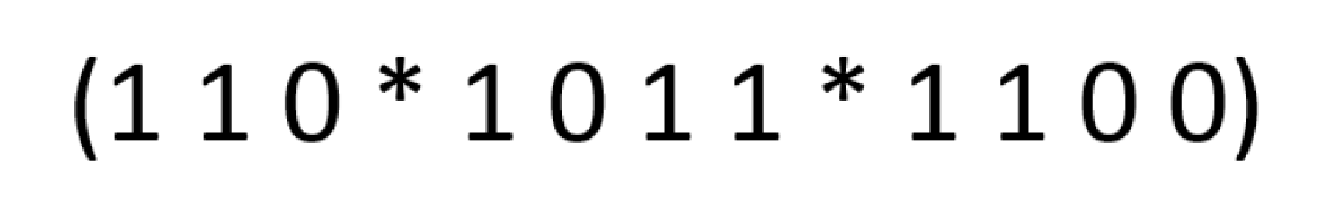
\epsfig{file=mutation.eps,height=0.4cm,width=4cm}
\end{center}

The evolution usually starts from a population of randomly generated individuals, 
and is an iterative process, with the population in each iteration called a generation.
\\\newline
\textbf{\large Initial population}
\begin{center}
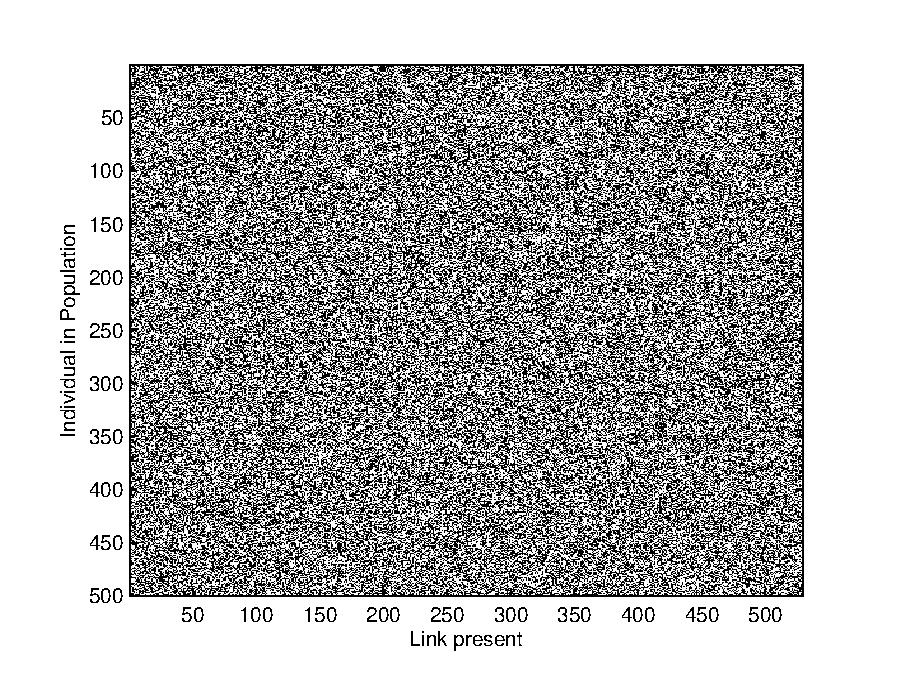
\epsfig{file=initial_population.eps,height=4cm,width=4cm}
\end{center}

For each individual, we evaluate a fitness function. Our fitness function is defined as follows :
Firs we compute the standard page rank of the individual matching mesh, which is defined as follows :
The first stage is the page rank initialisation for all our nodes:
\begin{equation}
\forall u \ PR\left(u\right)=\frac{1}{N}
\end{equation} 
We then iterate to find the fixed point solutions of the well know equation :
\begin{equation}
PR\left(u\right)= \frac{\left(1-c\right)}{N} + c \times \sum_{v \rightarrow u}\frac{PR\left(v\right)}{card\left(\left\{v\rightarrow u\right\}\right)}
\end{equation}


In each generation, the fitness of every individual in the population is evaluated; 
the fitness is usually the value of the objective function in the optimization problem being solved.
 
 The more fit individuals are stochastically selected from the current population, 
and each individual's genome is modified (recombined and possibly randomly mutated) to form a new generation. 
The new generation of candidate solutions is then used in the next iteration of the algorithm. 


Commonly, the algorithm terminates when either a maximum number of generations has been produced, 
or a satisfactory fitness level has been reached for the population.


\begin{equation}
\max_{\left(G_{ij}\right)  \in \left\{0,1\right\}^{N\times N}}\left\{ \sum^{N}_{i=1} trafic\left(X_i\right)\times PR(X_i)\right\}
\end{equation}
 \\\newline
Categorization of our links :

\textbf{\large Links categorization}
\begin{center}
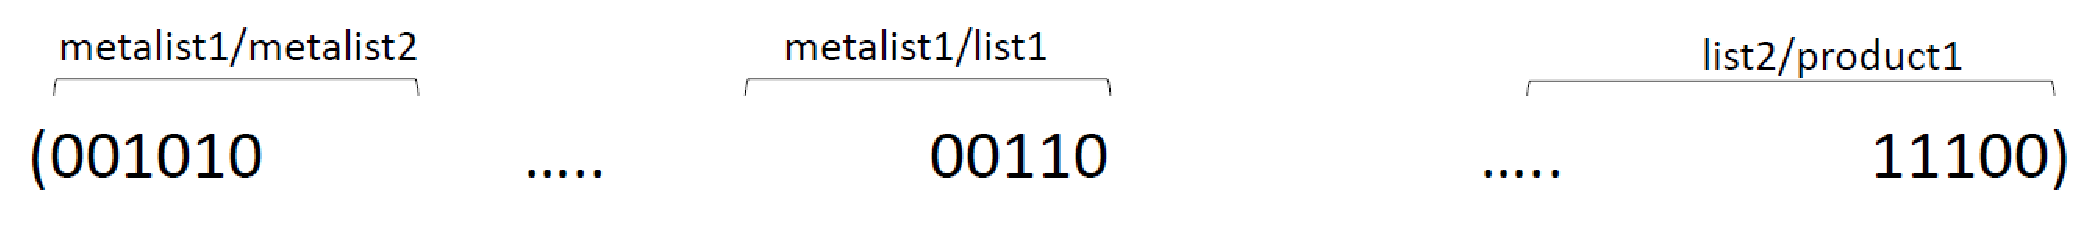
\epsfig{file=links_categorization.eps,height=1cm,width=6cm}
\end{center}

\textbf{\large Population at convergence}
\begin{center}
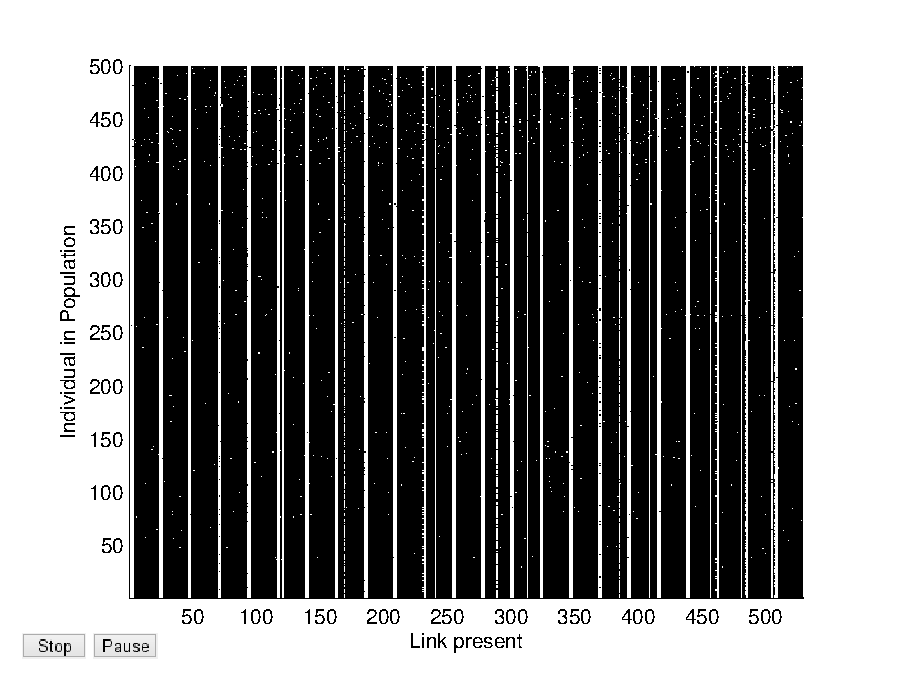
\epsfig{file=converged_population.eps,height=4cm,width=4cm}
\end{center}
\textbf{\large Best chromosome fitness function evolution}
\begin{center}
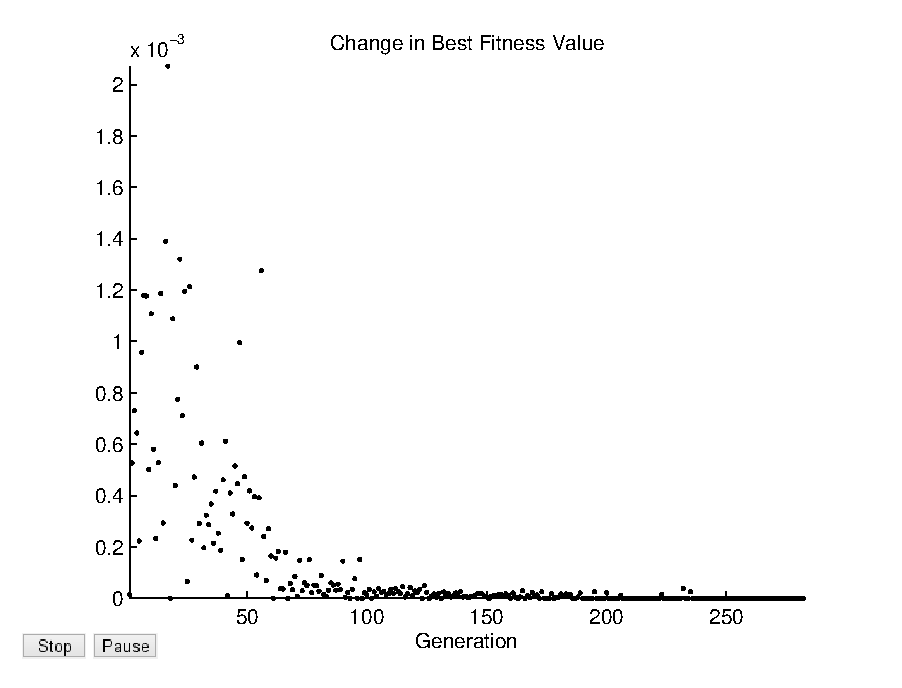
\epsfig{file=best_element_evolution.eps,height=4cm,width=4cm}
\end{center}

\section{Big data implementaino}
%\lipsum
%A citation example: \cite{donald1999art}.

\bibliographystyle{plain}
\bibliography{biblio}
\end{document}
